\documentclass[tikz,border=10pt]{standalone}
\usetikzlibrary{calc}
% Scale s = 0.021333 cm/px, origin at O (224.4,222.1), y flipped
\begin{document}
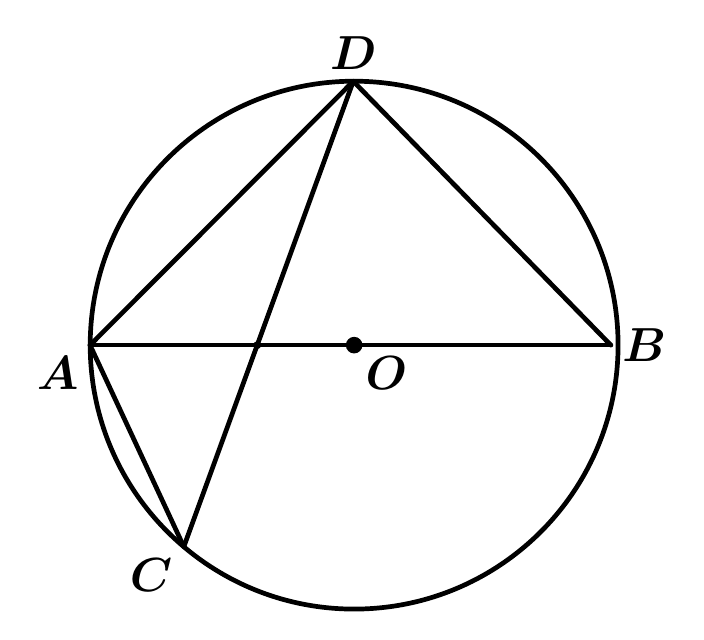
\begin{tikzpicture}[line width=1.7pt, line join=round, line cap=round,
  % labels: same size, bold math
  lbl/.style={font=\fontsize{18}{21.6}\selectfont\boldmath}]
  % Points (cm)
  \coordinate (O) at (0,0);
  \coordinate (A) at (-3.354,0);
  \coordinate (B) at (3.260,0);
  \coordinate (D) at (-0.011,3.351);
  \coordinate (C) at (-2.163,-2.560);
  \coordinate (E) at (-1.231,0);

  % Circle, radius 157.1 px
  \draw (O) circle (3.352);

  % Diameter AB
  \draw (A) -- (B);

  % Triangle segments
  \draw (D) -- (A);
  \draw (D) -- (B);
  \draw (D) -- (C);
  \draw (A) -- (C);

  % Intersection point E on AB
  \fill (E) circle (0.05);

  % Centre O: filled dot enlarged from 2.5pt to 3pt radius (~5 px in original)
  \fill (O) circle (3pt);

  % Labels
  \node[lbl, below left] at (A) {$A$};
  \node[lbl, right] at (B) {$B$};
  \node[lbl, above] at (D) {$D$};
  \node[lbl, below left] at (C) {$C$};
  \node[lbl, below right] at (O) {$O$};
\end{tikzpicture}
\end{document}